\noindent\begin{minipage}{7cm}
\begin{description}
\item[Objectif :] comprendre la récursivité.
\item[Syntaxe \python :] \mbox{}
\begin{Verbatim}
def fonction(entrées) :
    ...
    s = fonction(autres entrées)
    ...
    return sorties
\end{Verbatim}
\end{description}
\end{minipage}
\mbox{}\hfill
\begin{minipage}{5cm}
\centerline{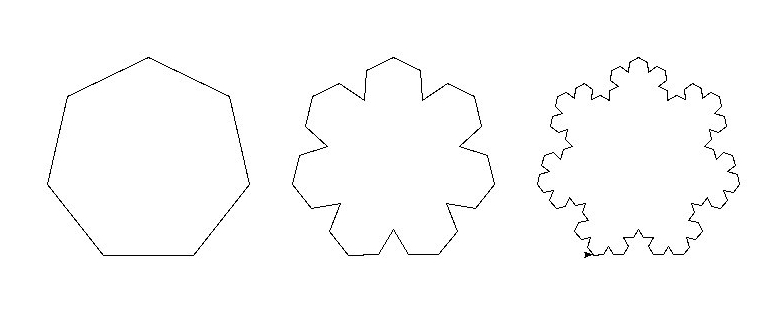
\includegraphics[width=5cm]{flocon2.jpg}}
\centerline{Flocons de Koch}
\end{minipage}
%\begin{tabular}{c}
%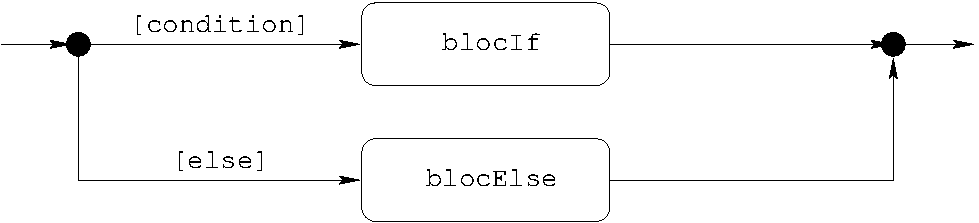
\includegraphics[width=6.5cm]{uml1.pdf}\\[3mm]
%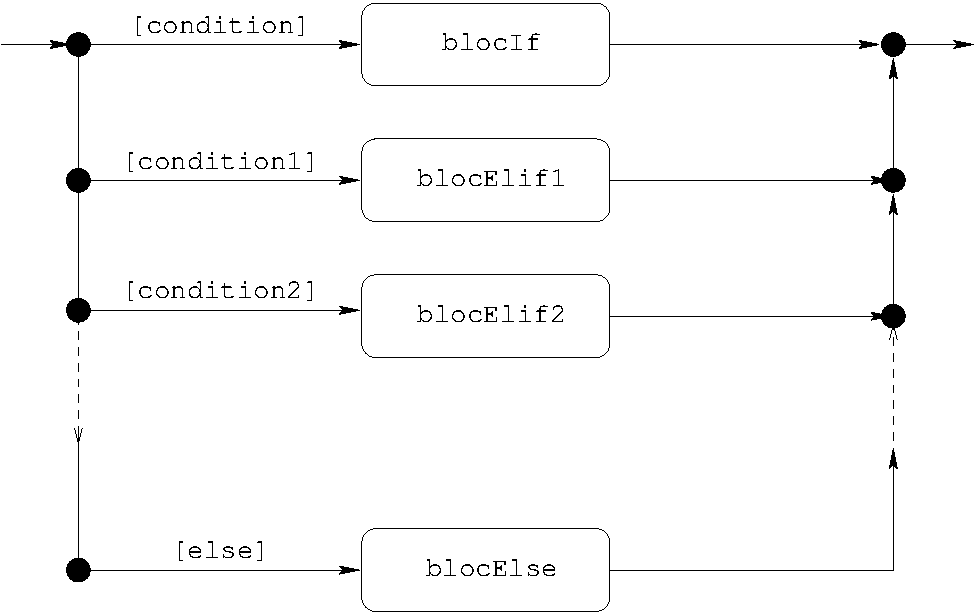
\includegraphics[width=6.5cm]{uml3.pdf}
%\end{tabular}

%-------------------------------------------------------------------------
\subsection{Exemple}
%-------------------------------------------------------------------------

\paragraph{Enoncé :} 
Les « tours de Hanoï » est un jeu imaginé par le mathématicien 
français Édouard Lucas (1842-1891). Il 
consiste à déplacer $n$ disques de diamètres différents d'une 
tour de « départ~» à une tour d'« arrivée » en passant par une 
tour « intermédiaire » et ceci en un minimum de coups, 
tout en respectant les règles suivantes :
\begin{itemize}
\item on ne peut déplacer qu'un disque à la fois;
\item on ne peut placer un disque que sur un autre disque 
	plus grand que lui ou sur une tour vide.
\end{itemize}
Dans l'état initial, les $n$ disques sont placés sur la tour
« départ ». Dans l'état final, tous les disques se retrouvent
placés dans le même ordre sur la tour « arrivée ».
\vspace*{3mm}

\noindent\begin{minipage}{7cm}
{Etat initial : $n=3$}\\[1mm]
\centerline{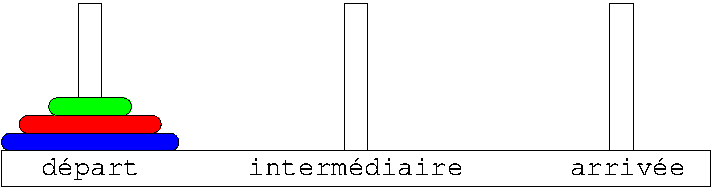
\includegraphics[width=7cm]{hanoi.pdf}}
\end{minipage}
\hfill
\begin{minipage}{7cm}
{Etat final : $n=3$}\\[1mm]
\centerline{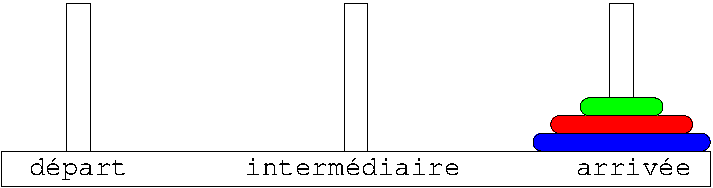
\includegraphics[width=7cm]{hanoi1.pdf}}
\end{minipage}
\vspace*{3mm}

\paragraph{Méthode :} On cherchera à mettre en évidence une relation de récurrence
entre le jeu à $n$ disques et le jeu à $n-1$ disques.


%\noindent\begin{minipage}{6cm}
%\textbf{Etat intermédiaire a:}\\
%\centerline{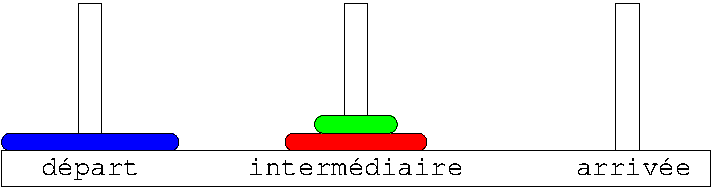
\includegraphics[width=6cm]{../../../v2/fig/hanoi2.pdf}}
%\end{minipage}
%\hfill
%\begin{minipage}{6cm}
%\textbf{Etat intermédiaire b:}\\
%\centerline{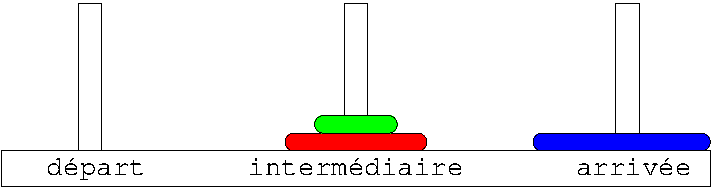
\includegraphics[width=6cm]{../../../v2/fig/hanoi3.pdf}}
%\end{minipage}

\begin{question}[« tours de Hanoï » : à la main]
Résoudre {\em à la main} le problème des tours de Hanoï à $n$ disques
successivement pour $n=1$, $n=2$ et $n=3$.
\end{question}

\begin{question}[« tours de Hanoï » : relation de récurrence]\mbox{}
\begin{enumerate}
\item Trouver une relation de récurrence entre le problème des tours de Hanoï à $n=4$ disques
	avec celui à $n=3$ disques.
\item Généraliser à un nombre de disques $n$ quelconque.
	En déduire qu'il faut effectuer $(2^n - 1)$ déplacements de disque pour déplacer $n$
	disques de la tour « départ » à la tour « arrivée ».
\item Proposer un algorithme pour résoudre le problème des tours de Hanoï 
	qui consiste à déplacer $n$ disques d'une tour de «~départ~» $(d)$ à une 
	tour d'«~arrivée~» $(a)$ en passant par une tour «~intermédiaire~» $(i)$.
\end{enumerate}
\end{question}

%-------------------------------------------------------------------------
\subsection{Généralisation}
%-------------------------------------------------------------------------
Une fonction est dite récursive si elle s'appelle elle-même : on parle 
alors d'appel récursif de la fonction.
Un appel récursif terminal est un appel récursif dont le résultat est celui 
retourné par la fonction. En d'autres termes, si dans le corps d'une fonction, 
un appel récursif est placé de telle façon que son exécution n'est jamais suivi 
par l'exécution d'une autre instruction de la fonction, cet appel est dit récursif
à droite ou récursif terminal.
A contrario, un appel récursif non terminal est 
un appel récursif dont le résultat n'est pas celui retourné par la fonction.


\begin{question}[récursivité : exécution d'une fonction récursive]\mbox{}\\
\noindent\begin{minipage}[t]{7.5cm}
On condidère la procédure récursive \texttt{f} définie ci-contre.
\begin{enumerate}
\item Qu'affichent les appels suivants ?
\begin{itemize}
\item[\texttt{>{>}>}] \texttt{f(0,'d','i','a')} ?
\item[\texttt{>{>}>}] \texttt{f(1,'d','i','a')} ?
\item[\texttt{>{>}>}] \texttt{f(2,'d','i','a')} ?
\item[\texttt{>{>}>}] \texttt{f(3,'d','i','a')} ?
\end{itemize}
\end{enumerate}
\end{minipage}
\hfill
\begin{minipage}[t]{7cm}\em
\begin{lstlisting}
def f(n,d,i,a) :
    if n > 0 :
        f(n-1,d,a,i)
        print(d,'->',a)
        f(n-1,i,d,a)
    return
\end{lstlisting}
\end{minipage}
\begin{enumerate}\setcounter{enumi}{1}
\item Vérifier que cette fonction \texttt{f} exécute correctement les 
	déplacements des $n$ disques des tours de Hanoï pour $n=0$, $n=1$, 
	$n=2$ et $n=3$ respectivement.
\item Dans le code précédent, qu'est-ce qui permet d'arrêter la récursivité ?
\end{enumerate}
\end{question}

Pour définir une fonction récursive, il faut disposer d'une relation de récurrence et d'un
cas particulier (clause d'arrêt).

\begin{question}[récursivité : fonction factorielle]
Définir une fonction récursive qui calcule la fonction factorielle $(n!)$.
Préciser la relation de récurrence et la clause d'arrêt.
\end{question}

\begin{question}[récursivité : plus grand commun diviseur]
Définir une fonction récursive qui calcule le plus grand commun diviseur $d$ de 2
entiers $a$ et $b$ : ${pgcd}(a,b) = {pgcd}(b,a\%b) = {pgcd}(d,0) = d$.
Préciser la relation de récurrence et la clause d'arrêt.
\end{question}

Quel que soit le problème à résoudre, on a le choix entre l'écriture d'une fonction 
itérative et celle d'une fonction récursive. Si le problème admet une décomposition 
récurrente naturelle, le programme récursif est alors une simple adaptation de la 
décomposition choisie. C'est le cas des fonctions \texttt{hanoi}, \texttt{factorielle} et \texttt{pgcd} par exemple.

L'approche récursive présente cependant des inconvénients :
certains langages n'admettent pas la récursivité (comme le langage machine !)
et elle est souvent coûteuse en mémoire comme en temps d'exécution. 
On peut pallier ces inconvénients en transformant la fonction récursive 
en fonction itérative : c'est toujours possible.

\begin{question}[récursivité : récursivité $\rightarrow$ itération]
Comparer les versions récursive et itérative de la fonction qui calcule
le plus grand commun diviseur $d$ de 2 entiers $a$ et $b$.
Montrer qu'on peut passer de la version récursive à la version itérative
en effectuant la transformation de code suivante :
\vspace*{3mm}

\noindent\begin{minipage}{7cm}
\begin{lstlisting}
def f(x) :
  if cond : return y
  else : 
    instructions
  return f(g(x))
\end{lstlisting}
\end{minipage}
\hfill$\rightarrow$\hfill
\begin{minipage}{7cm}
\begin{lstlisting}
def f(x) :
  while not cond :
    instructions
    x = g(x)
  return y
\end{lstlisting}
\end{minipage}
\vspace*{3mm}

\noindent où \texttt{x} représente ici la liste des arguments de la fonction
\texttt{f},
\texttt{cond} une condition portant sur \texttt{x}, 
\texttt{instructions} un bloc d'instructions qui constituent
le traitement de base de la fonction \texttt{f}, 
\texttt{g(x)} une transformation des arguments et \texttt{return y}
l'instruction de terminaison (clause d'arrêt) de la récurrence.
\end{question}

La méthode précédente ne s'applique qu'à la récursivité terminale.
Une méthode générale existe pour transformer une fonction récursive
quelconque en une fonction itérative équivalente. En particulier,
elle est mise en \oe uvre dans les compilateurs car le langage machine 
n'admet pas la récursivité. Cette méthode générale fait appel à la notion 
de pile pour sauvegarder le contexte des appels récursifs. 

%-------------------------------------------------------------------------
\subsection{Applications}
%-------------------------------------------------------------------------

\begin{question}[récursivité : fonction d'Ackerman]
Définir une fonction récursive qui calcule la fonction d'Ackerman : 
$$
{f : N^2 \rightarrow N}\ 
\left\{\begin{array}{lll}
f{(0,n)} & = & n+1\\
f{(m,0)} & = & f{(m-1,1)}\mbox{\ si\ } m > 0\\
f{(m,n)} & = & f{(m-1,f{(m,n-1)})}\mbox{\ si\ } m > 0, n > 0
\end{array}\right.
$$
\end{question}

\begin{question}[récursivité : coefficients du binôme]
Définir une fonction récursive qui calcule les coefficients du binôme 
$\displaystyle (a+b)^n = \sum_{k=0}^n \frac{n!}{k!(n-k)!}a^{n-k}b^k = \sum_{k=0}^n C_n^k a^{n-k}b^k$ où le coefficient du binôme $\displaystyle C_n^k$ représente le nombre de combinaisons de $k$ parmi $n$ :
$\displaystyle C_n^k = \frac{n!}{k!(n-k)!} = \left(\begin{array}{c}
n\\k
\end{array}\right)$.
\end{question}

\begin{question}[récursivité : flocons de Koch]\mbox{}

\noindent \begin{minipage}[t]{7.5cm}
On s'intéresse ici aux programmes dont l'exécution produit des dessins
à l'aide de la tortue \logo.
On considère la procédure \texttt{draw} ci-contre.
\begin{enumerate}
\item Dessiner le résultat des appels \texttt{draw(n,900)} 
	respectivement pour \texttt{n = 0}, \texttt{n = 1}, \texttt{n = 2} et \texttt{n = 3}. 
	A chaque appel, le crayon est initialement en $(0,0)$ avec une direction de $0$.
\item Définir une fonction \texttt{koch} qui dessine les flocons de Koch présentés
	sur la figure placée en exergue de la section \ref{sec:recursivite}.
\end{enumerate}
\end{minipage}
\hfill
\begin{minipage}[t]{7cm}
\begin{lstlisting}
def draw(n,d) :
  if n == 0 : forward(d)
  else :
    draw(n-1,d/3)
    left(60)
    draw(n-1,d/3)
    right(120)
    draw(n-1,d/3)
    left(60)
    draw(n-1,d/3)
  return
\end{lstlisting}
\end{minipage}
\end{question}

%-------------------------------------------------------------------------
\subsection{Entraînement}
%-------------------------------------------------------------------------

%-------------------------------------------------------------------------
\subsubsection{Enoncé}\label{f2f3}
%-------------------------------------------------------------------------
\paragraph{Objectif :} On considère la notion d'arbre binaire. Un arbre binaire
est soit vide, soit composé de 3 éléments :
une racine, un arbre binaire \texttt{Gauche} et un arbre binaire \texttt{Droite}.
L'arbre binaire vide sera représenté ici par la liste vide (\texttt{[]}), l'arbre binaire
non vide par une liste de 3 éléments (\texttt{[racine,Gauche,Droite]}) où \texttt{Gauche}
et \texttt{Droite} sont eux-mêmes des arbres binaires et \texttt{racine} de type quelconque.


\noindent \begin{minipage}{11cm}
Ainsi, l'arbre binaire ci-contre
est représenté par la liste :\\
\texttt{[1, [2,[],[]], [3,[],[4,[],[]]]]}.
\end{minipage}
\hfill
\begin{minipage}{4cm}
\fbox{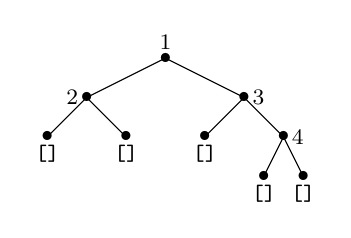
\begin{tikzpicture}[scale=0.5]\footnotesize
\draw (3,4) node {$\bullet$};
\draw (3,4) node[above] {$1$};
\draw (1,3) node {$\bullet$};
\draw (1,3) node[left] {$2$};
\draw (5,3) node {$\bullet$};
\draw (5,3) node[right] {$3$};
\draw (0,2) node {$\bullet$};
\draw (0,2) node[below] {\texttt{[]}};
\draw (2,2) node {$\bullet$};
\draw (2,2) node[below] {\texttt{[]}};
\draw (4,2) node {$\bullet$};
\draw (4,2) node[below] {\texttt{[]}};
\draw (6,2) node {$\bullet$};
\draw (6,2) node[right] {$4$};
\draw (5.5,1) node {$\bullet$};
\draw (5.5,1) node[below] {\texttt{[]}};
\draw (6.5,1) node {$\bullet$};
\draw (6.5,1) node[below] {\texttt{[]}};
\draw (3,4) -- (5,3);
\draw (3,4) -- (1,3);
\draw (1,3) -- (0,2);
\draw (1,3) -- (2,2);
\draw (5,3) -- (4,2);
\draw (5,3) -- (6,2);
\draw (6,2) -- (5.5,1);
\draw (6,2) -- (6.5,1);
\end{tikzpicture}}
\end{minipage}
\vspace*{3mm}

Les deux fonctions récursives \texttt{infix} et \texttt{postfix} ci-dessous permettent
d'afficher les éléments d'un arbre binaire (\texttt{0} pour l'arbre vide) de deux
manières différentes, respectivement en notation infixée et postfixée.

\noindent
%\begin{minipage}[t]{4cm}\footnotesize
%\begin{lstlisting}
%def f1(t) :
% if t != [] :
%  print(t[0],end=' ')
%  f1(t[1])
%  f1(t[2])
% else : 
%  print(0,end=' ')
% return
%\end{lstlisting}
%\end{minipage}
%\hfill
\begin{minipage}[t]{7cm}
\begin{lstlisting}
def infix(t) :
  if t != [] :
    infix(t[1])
    print(t[0],end=' ')
    infix(t[2])
  else : 
    print(0,end=' ')
  return
\end{lstlisting}
\end{minipage}
\hfill
\begin{minipage}[t]{7cm}
\begin{lstlisting}
def postfix(t) :
  if t != [] :
    postfix(t[1])
    postfix(t[2])
    print(t[0],end=' ')
  else : 
    print(0,end=' ')
  return
\end{lstlisting}
\end{minipage}
\vspace*{2mm}

\noindent
\begin{minipage}[t]{7cm}\footnotesize
\begin{Verbatim}
>>> t = [1, [2,[],[]], [3,[],[4,[],[]]]]
>>> infix(t)
0 2 0 1 0 3 0 4 0 
\end{Verbatim}
\end{minipage}
\hfill
\begin{minipage}[t]{7cm}\footnotesize
\begin{Verbatim}
>>> t = [1, [2,[],[]], [3,[],[4,[],[]]]]
>>> postfix(t)
0 0 2 0 0 0 4 3 1
\end{Verbatim}
\end{minipage}

\paragraph{Question :} Exécuter « à la main » les fonctions \texttt{infix} et \texttt{postfix} sur des arbres
binaires.

\paragraph{Vérification :} Représenter graphiquement l'arbre binaire et le parcourir
de manière infixée et postfixée pour comparer aux résultats obtenus par les fonctions
\texttt{infix} et \texttt{postfix}. Finalement, vérifier avec \python.

%-------------------------------------------------------------------------
\subsubsection{Exemple}
%-------------------------------------------------------------------------
On veut parcourir l'arbre binaire \texttt{t = [1,[2,[4,[],[]],[]],[3,[5,[],[]],[6,[],[7,[], []]]]]} de manière infixée (fonction \texttt{infix}) et de manière postfixée (fonction \texttt{postfix}).

\paragraph{Méthode :} En notation infixée, on commence par décrire le sous-arbre de gauche
\texttt{t[1]} (\texttt{= [[2,[4,[],[]],[]]]}), la racine \texttt{t[0]} (\texttt{= 1})
puis le sous-arbre de droite
\texttt{t[2]} (\texttt{= [3,[5,[],[]], [6,[],[7,[],[]]]]}). 
Le sous-arbre de gauche \texttt{t[1]} est lui même décrit
en commençant par son sous-arbre de gauche \texttt{t[1][1]} (\texttt{= [4,[],[]]}), 
la racine \texttt{t[1][0]} (\texttt{= 2}) puis son sous-arbre de droite \texttt{t[1][2]} 
(\texttt{= []}). Enfin le sous-arbre de gauche \texttt{t[1][1]} est décrit en commençant
par son sous-arbre de gauche \texttt{t[1][1][1]} (\texttt{= []}), sa racine \texttt{t[1][1][0]}
(\texttt{= 4}) puis son sous-arbre de droite \texttt{t[1][1][2]} (\texttt{= []}).
Lorsqu'un arbre est vide, on le décrit par \texttt{0}.
Ainsi, en notation infixée, le sous-arbre gauche \texttt{t[1]} 
(\texttt{= [[2,[4,[],[]],[]]]}) est représenté par
la séquence \texttt{0 4 0 2 0}. On procède de même avec le sous-arbre de droite
\texttt{t[2]} (\texttt{= [3,[5,[],[]],[6,[],[7,[],[]]]]}); ce qui conduit à la séquence
\texttt{0 5 0 3 0 6 0 7 0}. L'arbre \texttt{t} complet est donc décrit par la séquence
\texttt{0 4 0 2 0 1 0 5 0 3 0 6 0 7 0} en notation infixée.

En notation postfixée, on commence par décrire le sous-arbre de gauche 
\texttt{t[1]} (\texttt{= [[2,[4,[], []],[]]]}), le sous-arbre de droite
\texttt{t[2]} (\texttt{= [3,[5,[],[]],[6,[],[7,[],[]]]]}), puis la racine \texttt{t[0]} (\texttt{= 1}). 
Le sous-arbre de gauche \texttt{t[1]} est lui même décrit
en commençant par son sous-arbre de gauche \texttt{t[1][1]} (\texttt{= [4,[],[]]}), 
son sous-arbre de droite \texttt{t[1][2]} (\texttt{= []}) puis la racine \texttt{t[1][0]} (\texttt{= 2}). Enfin le sous-arbre de gauche \texttt{t[1][1]} est décrit en commençant
par son sous-arbre de gauche \texttt{t[1][1][1]} (\texttt{= []}), son sous-arbre de droite \texttt{t[1][1][2]} (\texttt{= []}) puis sa racine \texttt{t[1][1][0]}
(\texttt{= 4}).
Lorsqu'un arbre est vide, on le décrit par \texttt{0}.
Ainsi, en notation postfixée, le sous-arbre gauche \texttt{t[1]} 
(\texttt{= [[2,[4,[],[]],[]]]}) est représenté par
la séquence \texttt{0 0 4 0 2}. On procède de même avec le sous-arbre de droite
\texttt{t[2]} (\texttt{= [3,[5,[],[]],[6,[],[7,[],[]]]]}); ce qui conduit à la séquence
\texttt{0 0 5 0 0 0 7 6 3}. L'arbre \texttt{t} complet est donc décrit par la séquence
\texttt{0 0 4 0 2 0 0 5 0 0 0 7 6 3 1} en notation postfixée.

\paragraph{Résultats :} Les résultats sont reportés dans le tableau ci-dessous.
$$\begin{tabular}{l@{ : }l@{ $\rightarrow$ }r}
\multicolumn{3}{c}{\texttt{t = [1,[2,[4,[],[]],[]],[3,[5,[],[]],[6,[],[7,[],[]]]]]}}\\
\hline
notation infixée   & \texttt{infix(t)}   & \texttt{0 4 0 2 0 1 0 5 0 3 0 6 0 7 0} \\
notation postfixée & \texttt{postfix(t)} & \texttt{0 0 4 0 2 0 0 5 0 0 0 7 6 3 1}
\end{tabular}$$

\paragraph{Vérification :} On vérifie selon deux méthodes :
\begin{itemize}
\item en s'aidant de la représentation graphique de l'arbre binaire,
\item en exécutant le code sous \python.
\end{itemize}
\vspace*{3mm}

\noindent
\begin{minipage}{8cm}
\begin{enumerate}
\item La représentation binaire ci-contre permet de se faire 
	visuellement une meilleure idée de l'arbre binaire \texttt{t}
	et de repérer plus facilement les sous-arbres gauche et droite 
	à tous les niveaux de l'arbre. On vérifie aisément par exemple
	que le sous-arbre de gauche est représenté par la séquence \texttt{0 4 0 2 0}
	en notation infixée et par la séquence \texttt{0 0 4 0 2} en notation postfixée, 
	et ainsi de suite\ldots
\end{enumerate}
\end{minipage}
\hfill
\begin{minipage}{7cm}
\fbox{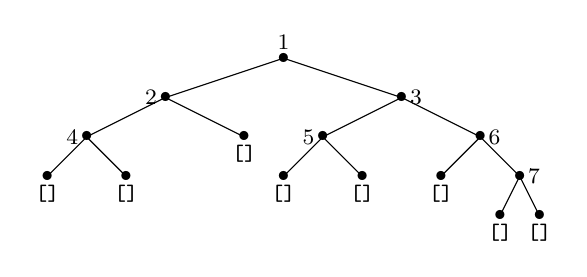
\begin{tikzpicture}[scale=0.5]\footnotesize
\draw (6,4) node {$\bullet$};
\draw (6,4) node[above] {$1$};
\draw (3,3) node {$\bullet$};
\draw (3,3) node[left] {$2$};
\draw (9,3) node {$\bullet$};
\draw (9,3) node[right] {$3$};
\draw (1,2) node {$\bullet$};
\draw (1,2) node[left] {$4$};
\draw (5,2) node {$\bullet$};
\draw (5,2) node[below] {\texttt{[]}};
\draw (7,2) node {$\bullet$};
\draw (7,2) node[left] {$5$};
\draw (11,2) node {$\bullet$};
\draw (11,2) node[right] {$6$};
\draw (0,1) node {$\bullet$};
\draw (0,1) node[below] {\texttt{[]}};
\draw (2,1) node {$\bullet$};
\draw (2,1) node[below] {\texttt{[]}};
\draw (6,1) node {$\bullet$};
\draw (6,1) node[below] {\texttt{[]}};
\draw (8,1) node {$\bullet$};
\draw (8,1) node[below] {\texttt{[]}};
\draw (10,1) node {$\bullet$};
\draw (10,1) node[below] {\texttt{[]}};
\draw (12,1) node {$\bullet$};
\draw (12,1) node[right] {$7$};
\draw (11.5,0) node {$\bullet$};
\draw (11.5,0) node[below] {\texttt{[]}};
\draw (12.5,0) node {$\bullet$};
\draw (12.5,0) node[below] {\texttt{[]}};
\draw (6,4) -- (3,3);
\draw (6,4) -- (9,3);
\draw (3,3) -- (1,2);
\draw (3,3) -- (5,2);
\draw (9,3) -- (11,2);
\draw (9,3) -- (7,2);
\draw (1,2) -- (0,1);
\draw (1,2) -- (2,1);
\draw (7,2) -- (6,1);
\draw (7,2) -- (8,1);
\draw (11,2) -- (10,1);
\draw (11,2) -- (12,1);
\draw (12,1) -- (12.5,0);
\draw (12,1) -- (11.5,0);
\end{tikzpicture}}
\end{minipage}

\begin{enumerate}\setcounter{enumi}{1}
\item L'exécution sous \python{} confirme nos premiers résultats :

\begin{Verbatim}
>>> t = [1,[2,[4,[],[]],[]],[3,[5,[],[]],[6,[],[7,[],[]]]]]
>>> infix(t)
0 4 0 2 0 1 0 5 0 3 0 6 0 7 0 
>>> postfix(t)
0 0 4 0 2 0 0 5 0 0 0 7 6 3 1 
\end{Verbatim}
\end{enumerate}

%-------------------------------------------------------------------------
\subsubsection{Questions}
%-------------------------------------------------------------------------
On reprend ici les fonctions \texttt{infix} et \texttt{postfix} définies plus haut 
(section \ref{f2f3}). Exécuter à la main les appels suivants.

\begin{enumerate}
\item \texttt{>{>}> infix([1, [3, [5,[],[]], []] , [2, [], [4,[],[]]]])}
\item \texttt{>{>}> postfix([1, [3, [5,[],[]], []] , [2, [], [4,[],[]]]])}

\item \texttt{>{>}> infix([2, [4, [6,[],[]], []] , [1, [], [3,[],[]]]])}
\item \texttt{>{>}> postfix([2, [4, [6,[],[]], []] , [1, [], [3,[],[]]]])}

\item \texttt{>{>}> infix([1, [3, [], [5,[],[]]] , [2, [4,[],[]], []]])}
\item \texttt{>{>}> postfix([1, [3, [], [5,[],[]]] , [2, [4,[],[]], []]])}

\item \texttt{>{>}> infix([2, [4, [], [6,[],[]]] , [1, [3,[],[]], []]])}
\item \texttt{>{>}> postfix([2, [4, [], [6,[],[]]] , [1, [3,[],[]], []]])}

\item \texttt{>{>}> infix([1, [3, [5,[],[]], [4,[],[]]] , [2, [], []]])}
\item \texttt{>{>}> postfix([1, [3, [5,[],[]], [4,[],[]]] , [2, [], []]])}

\item \texttt{>{>}> infix([2, [4, [], []] , [1, [], [6,[],[3,[],[]]]]])}
\item \texttt{>{>}> postfix([2, [4, [], []] , [1, [], [6,[],[3,[],[]]]]])}

\item \texttt{>{>}> infix([1, [], [2, [], [3, [5,[],[]], [4,[],[]]]]])}
\item \texttt{>{>}> postfix([1, [], [2, [], [3, [5,[],[]], [4,[],[]]]]])}

\item \texttt{>{>}> infix([2, [4, [], []] , [1, [], [6,[],[3,[],[]]]]])}
\item \texttt{>{>}> postfix([2, [4, [], []] , [1, [], [6,[],[3,[],[]]]]])}

\item \texttt{>{>}> infix([1, [2, [4,[],[]], [3, [5,[],[]], []]], []])}
\item \texttt{>{>}> postfix([1, [2, [4,[],[]], [3, [5,[],[]], []]], []])}

\item \texttt{>{>}> infix([2, [], [1, [4, [], []], [6,[],[3,[],[]]]]])}
\item \texttt{>{>}> postfix([2, [], [1, [4, [], []], [6,[],[3,[],[]]]]])}

\item \texttt{>{>}> infix([5, [3, [1,[],[]], []] , [4, [], [2,[],[]]]])}
\item \texttt{>{>}> postfix([5, [3, [1,[],[]], []] , [4, [], [2,[],[]]]])}

\item \texttt{>{>}> infix([6, [4, [2,[],[]], []] , [3, [], [1,[],[]]]])}
\item \texttt{>{>}> postfix([6, [4, [2,[],[]], []] , [3, [], [1,[],[]]]])}
\end{enumerate}

%-------------------------------------------------------------------------
\subsection{Révisions}
%-------------------------------------------------------------------------

$$\begin{tabular}{|ll@{ : }l|}
\hline
\textbf{Cours} & \cite{cours} & chapitre 3, section 3.3 \\
\textbf{TD}    & \cite{td}    & exercices 3.9 à 3.12, 3.16 à 3.19 \\
\hline
\end{tabular}$$

